\documentclass{article}
\usepackage{iclr2026_conference,times}
\input{math_commands.tex}
\usepackage{amsmath}
\usepackage{amssymb}
\usepackage{amsthm}
\usepackage{booktabs}
\usepackage{graphicx}
\usepackage{multirow}
\usepackage{array}
\usepackage{longtable}
\usepackage{tabularx}
\usepackage{xcolor}
\usepackage{url}
\usepackage[
  colorlinks=false,
  pdfborder={0 0 1.6},
  citebordercolor={1 0.10 0.00},
  linkbordercolor={0.00 0.30 1.00},
  urlbordercolor={0.00 0.55 0.20}
]{hyperref}

\newtheorem{proposition}{Proposition}
\newtheorem{assumption}{Assumption}
\newtheorem{definition}{Definition}
\newcommand{\method}{RC-FEV}
\newcommand{\energy}{\mathcal{E}}
\newcommand{\actions}{\mathcal{A}}
\newcommand{\branches}{\mathcal{B}}
\newcommand{\tokens}{\mathcal{Z}}
\newcommand{\features}{\phi}
\newcommand{\cvar}{\operatorname{CVaR}}

\title{Robust Calibrated Force-Effect Vocabularies for Cross-Embodiment Contact-Rich Manipulation}
\author{Anonymous Authors}

\begin{document}
\maketitle

\begin{abstract}
Cross-embodiment robot learning is usually evaluated through policy transfer, representation sharing, or large-scale behavior cloning. This paper studies a narrower but operationally important question: can an embodiment-normalized vocabulary of contact force/effect modes improve one-step contact-rich action selection under pusher morphology, actuator, object-mass, friction, and actuation-noise shifts? We rebuild an earlier four-page scaffold into a full MuJoCo benchmark and evaluate a robust calibrated force-effect vocabulary (\method). The benchmark uses 240 source fitting tasks, 10 learned force/effect tokens, 8 random seeds, 20 episodes per seed/split, 10 stress splits, 11 main action selectors, and 17,600 frozen main evaluation rows; two hostile ablation splits add 3,520 rows. \method combines normalized contact descriptors, tokenized source-branch outcomes, a CVaR source-energy term, a worst-branch robust anchor, and lightweight online residual calibration. The final result is useful but not submission-clean: \method beats weak transfer baselines and the previous CEFV v4 vocabulary in aggregate, and slightly improves over robust and CVaR domain-randomized MPC in aggregate energy, but multiple ablations match or slightly beat the full method on the frozen ablation gate. The correct terminal decision is therefore \textbf{STRONG REVISE}. The contribution of this version is not a polished state-of-the-art claim; it is a reproducible, hostile-review benchmark, a clearer theory of when force/effect tokenization should help, and an honest evidence package that identifies exactly what remains missing before an ICLR-main submission.
\end{abstract}

\section{Introduction}

Robots that execute visually similar contact actions can produce sharply different physical effects. A small stiff pusher, a large compliant pusher, a high-gain heavy pusher, and a weak actuator can all be commanded to ``push the box toward the target.'' The commanded path may be the same, but the induced normal impulse, tangential slip, yaw, contact duration, and final progress can differ enough to invalidate action transfer. This is the practical tension behind cross-embodiment manipulation: action coordinates are easy to share, while contact effects are not.

Large robot datasets and transformer policies have made cross-embodiment learning a central target in modern robotics \citep{brohan2023rt1,brohan2023rt2,openx2023}. Sim-to-real and domain randomization methods make a complementary bet: train policies or model-based controllers under broad variation until they become robust to a family of dynamics \citep{tobin2017domain,peng2018sim,chebotar2019closing}. Model-based reinforcement learning and MPC further offer uncertainty-aware planning tools \citep{nagabandi2018neural,chua2018pets}. Those directions are important, but they do not directly answer a smaller representational question: when a contact primitive is being selected, should we reason in the original action coordinates, in raw forces, in model rollouts, or in a learned vocabulary of force/effect modes?

This paper investigates that question in a deliberately restricted setting. Each episode is a single controlled pushing primitive in MuJoCo \citep{todorov2012mujoco}. The agent chooses one candidate push from a compact action library. The pusher and object distribution shift across radius, pusher mass, actuator gain, damping, contact compliance, floor friction, object mass, and actuation noise. The task is not to solve all manipulation, but to test whether a discrete vocabulary of normalized contact outcomes can serve as a useful interface for selecting contact actions under embodiment shift.

The proposed method, robust calibrated force-effect vocabulary (\method), is a rebuilt version of a weaker earlier vocabulary selector. The earlier version showed a positive signal against geometry-only and raw-force baselines, but it was too small and did not survive comparison to robust domain-randomized MPC. The present paper fixes the evaluation standard first, then tests the method. The final protocol was frozen before the full run: 240 source fitting tasks, a 10-token vocabulary, 8 seeds, 20 episodes per seed/split, 10 main stress splits, 11 main methods, and two hostile ablation splits. The final run produced 17,600 main rows and 3,520 ablation rows. All reported numbers come from that frozen run.

The central result is mixed in a way that is valuable for development but unsafe for a main-conference acceptance claim. In aggregate, \method reaches 0.578 success and 0.1379 energy, beating geometry MPC, raw-force scalar transfer, continuous force regression, source-action transfer, CEFV v4, robust MPC, and CVaR MPC by small or large margins depending on the baseline. Against robust MPC the aggregate advantage is tiny: +0.0156 success and 0.0008 lower energy. Against CVaR MPC it is also tiny: +0.0138 success and 0.0002 lower energy. The ablation audit is more damaging. On the hostile ablation splits, variants without online adaptation, without embodiment normalization, without tangent/rotation features, without the robust anchor, or with a smaller vocabulary can match or slightly beat the full method on some metrics. That is the reason for the terminal decision: \textbf{STRONG REVISE}.

This manuscript is written to optimize for hostile review rather than pretty results. The main claims are intentionally narrow:

\begin{itemize}
\item A normalized force/effect vocabulary can improve contact-action selection over weak action-coordinate and raw-force transfer baselines in a controlled MuJoCo stress test.
\item Robust and CVaR domain-randomized MPC are strong baselines; the present method does not dominate them decisively.
\item The full mechanism is not isolated by the current ablations. Online calibration helps only modestly, and several simplified variants remain competitive.
\item The current artifact is a reproducible strong-revise package, not an ICLR-main-ready acceptance claim.
\end{itemize}

\section{Related Work}

\paragraph{Cross-embodiment robot learning.}
Large-scale robot learning has shifted the field from single-robot policies toward shared models that operate across tasks, scenes, and embodiments \citep{brohan2023rt1,brohan2023rt2,openx2023}. Those works show the value of scale and broad data support. They also make the evaluation bar higher for any narrow cross-embodiment paper: a new representation must show why it is not merely a small proxy for generic policy scaling. \method is not proposed as a replacement for large policies. It is a contact-action selection module that can be evaluated independently of image encoders, language conditioning, or dataset scale.

\paragraph{Sim-to-real and domain randomization.}
Domain randomization trains under randomized appearances or dynamics so that the learned controller transfers to unseen physical conditions \citep{tobin2017domain,peng2018sim}. Adaptive randomization closes the loop between observed deployment failures and future simulation distributions \citep{chebotar2019closing}. These methods motivate two strong baselines in our benchmark: robust domain-randomized MPC, which minimizes worst-branch source energy, and CVaR MPC, which minimizes the average of high-energy source branches. The point of including these baselines is to prevent a vocabulary method from winning only because the alternatives are weak.

\paragraph{Model-based control and uncertainty.}
Model-based reinforcement learning can be data-efficient when a learned dynamics model supports planning \citep{nagabandi2018neural,chua2018pets}. Classic model-based robotics has long used simulation and contact models for planning and control \citep{todorov2012mujoco,erez2015simulation}. Our setting is deliberately simpler than full learned dynamics: source branches are fixed MuJoCo models, candidate actions are short horizon pushes, and evaluation uses the true held-out branch. This makes the comparison sharper: if a force/effect vocabulary helps, it should help in action scoring, not because of unrelated perception or long-horizon policy effects.

\paragraph{Contact mechanics and force control.}
Contact-rich manipulation is governed by frictional interaction, compliance, and contact geometry. Stable pushing has a long mechanics literature \citep{lynch1996stable,mason2001mechanics}; impedance and operational-space control provide classical ways to regulate contact interactions \citep{hogan1985impedance,khatib1987operational}. \method is not a new contact controller. It uses a fixed push primitive and asks whether contact measurements can be compressed into reusable action-selection tokens.

\paragraph{Fast adaptation and meta-learning.}
Meta-learning and rapid adaptation methods aim to adjust behavior after limited deployment experience \citep{finn2017maml,kumar2021rma}. The online component of \method is far lighter: it maintains token and action-family residuals in a deployment stream. This keeps CPU and RAM cost small, but the final results show the downside of such a simple adaptation layer. Online calibration changes only a small number of decisions and does not isolate a large performance gain.

\paragraph{Risk-sensitive objectives.}
Worst-case and tail-risk objectives are natural for cross-embodiment transfer because average source performance can hide catastrophic mismatch. We therefore include robust and CVaR baselines, following the general risk-measure perspective of coherent risk and conditional value-at-risk \citep{artzner1999coherent,rockafellar2000optimization}. The full \method score also includes a robust anchor. The ablation results show that this anchor is useful but not sufficient to prove the entire vocabulary stack.

\paragraph{Novelty boundary.}
The novelty claimed here is not ``robot foundation model,'' ``new contact physics,'' or ``state-of-the-art manipulation.'' The narrow novelty boundary is a hostile evaluation of force/effect tokenization as an embodiment-normalized interface for contact-action selection. The final evidence supports the interface as useful, but not yet as decisive.

\section{Problem Setup}

\subsection{Embodiments, Objects, and Branches}

An episode samples a task
\[
  \tau = (e, o, x_0, g, \sigma)
\]
where $e$ is a pusher embodiment, $o$ is an object and floor-contact setting, $x_0$ is the initial box position, $g$ is the target, and $\sigma$ is the actuation-noise scale. An embodiment specifies pusher radius, pusher mass, actuator proportional gain, slide-joint damping, contact compliance, and pusher friction. An object setting specifies box mass and floor friction. A branch $b=(e,o)$ is a concrete simulation model.

The agent receives a finite action set $\actions(\tau)=\{a_1,\ldots,a_K\}$ with $K=45$. Each action is a short push parameterized by angle offset, lateral offset, and distance. The action library is intentionally compact. The benchmark is not testing continuous trajectory optimization; it is testing how to score a set of plausible contact primitives under embodiment shift.

\subsection{Outcome and Energy}

Executing action $a$ in branch $b$ produces an outcome
\[
  y = F_b(x_0,g,a,\epsilon),
\]
where $\epsilon$ captures actuation noise. The outcome includes final box position, yaw, normal and tangential contact impulse, peak contact forces, contact steps, effort, and failure flags. The scalar energy used for action selection and evaluation is
\[
  \energy(y) =
  d_{\mathrm{final}}(y,g)
  + 0.020\,\mathrm{effort}(y)
  + 0.035\,|\mathrm{yaw}(y)|
  + 0.220\,\mathrm{failure}(y).
\]
Lower energy is better. Success is reported separately as final distance at most 7.5 cm and no failure. The oracle upper bound selects the candidate with minimum true held-out energy; it is not available to deployable methods.

\subsection{Source Branch Library}

At test time, deployable methods do not directly evaluate candidate actions in the true held-out branch. Instead, they evaluate actions through a fixed source branch library $\branches=\{b_1,\ldots,b_M\}$ with $M=5$. For each candidate action $a$, the benchmark records source outcomes
\[
  \{F_{b_m}(x_0,g,a,0)\}_{m=1}^M.
\]
Baselines use these source outcomes in different ways: mean source energy, worst source energy, CVaR source energy, raw force scalar nearest-neighbor transfer, or learned force/effect tokens.

\section{Method: Robust Calibrated Force-Effect Vocabulary}

\subsection{Force/Effect Descriptors}

For each source rollout we compute a descriptor $\features(y,a,b)$. The full descriptor contains:

\begin{itemize}
\item log-normalized normal impulse;
\item log-normalized tangential impulse;
\item tangential impulse ratio;
\item contact-step fraction;
\item normalized peak normal and tangential contact force;
\item normalized progress toward the target;
\item final-distance ratio;
\item yaw magnitude;
\item sine and cosine of action angle offset;
\item lateral action offset normalized by pusher radius;
\item action distance normalized by pusher radius.
\end{itemize}

The normalization matters because raw forces are not comparable across pusher radii and actuator gains. A large compliant pusher can generate different absolute forces than a small stiff one while producing a similar useful contact mode. The intended role of the descriptor is to expose contact effects rather than raw actuator units.

\subsection{Vocabulary Fitting}

The source fitting stage samples 240 tasks over nominal, low-friction, heavy-object, high-friction, and actuation-noise regimes. Each task evaluates the 45 candidate actions on one source branch, producing 10,800 fitting rollouts. We standardize the descriptors and run deterministic $k$-means with $k=10$ \citep{lloyd1982least}. Each token $z\in\tokens$ stores its mean energy, standard deviation, success rate, and count.

We fit additional token models for ablations:

\begin{itemize}
\item a raw, unnormalized force vocabulary;
\item an action-only vocabulary;
\item a tangent/rotation-masked vocabulary;
\item a small vocabulary with four tokens.
\end{itemize}

These ablations are important because a vocabulary can appear useful for the wrong reason. If an action-only vocabulary performs as well as the full force/effect descriptor, then force measurements are not doing the claimed work.

\subsection{Candidate Scoring}

For a test task and candidate action $a$, each source branch produces an outcome descriptor and token assignment. Let $\hat{\energy}_{z_m}$ be the token mean energy for source branch $m$, optionally corrected by online residuals. Define
\[
  \mu_z(a)=\frac{1}{M}\sum_{m=1}^M \hat{\energy}_{z_m},
\]
and let $u_z(a)$ combine token energy dispersion, token uncertainty, and source-branch energy dispersion. Let
\[
  \bar{\energy}_{B}(a)=\frac{1}{M}\sum_{m=1}^M \energy(F_{b_m}(a)),
\]
\[
  \energy_{\max}(a)=\max_m \energy(F_{b_m}(a)),
\]
and
\[
  \cvar_{0.40}(a)
\]
be the mean of the worst 40 percent source energies. The calibrated score is
\[
\begin{aligned}
S_{\mathrm{cal}}(a) =
&0.38\,\cvar_{0.40}(a)
+0.22\,\mu_z(a)
+0.18\,\bar{\energy}_{B}(a)\\
&+0.07\,G(a)
+0.10\,u_z(a)
+0.30\,r_{\mathrm{act}}(a)
+0.08\,r_{\mathrm{mis}}(a),
\end{aligned}
\]
where $G(a)$ is a geometric target-distance heuristic, $r_{\mathrm{act}}$ is a lightweight online action-family residual, and $r_{\mathrm{mis}}$ is an online mismatch penalty scaled by source disagreement. The final score blends this calibrated score with the robust anchor:
\[
  S_{\method}(a)=\lambda(a)\energy_{\max}(a)+(1-\lambda(a))S_{\mathrm{cal}}(a).
\]
The weight $\lambda(a)$ is larger when token/source disagreement is high and decreases modestly as online evidence accumulates. The selected action is $\arg\min_a S_{\method}(a)$.

\subsection{Online Calibration}

The online state is intentionally small. It stores:

\begin{itemize}
\item token residuals keyed by discrete token id;
\item coarse action-family residuals keyed by angle-offset bin, lateral-offset bin, and distance family;
\item a global residual;
\item the last absolute prediction error.
\end{itemize}

After executing a selected action, the observed true energy updates the residual state. This is closer to a streaming calibration layer than to meta-learning. The design keeps memory nearly constant and CPU overhead negligible relative to MuJoCo rollouts. The final ablation results show that this lightness has a cost: online calibration is measurable but not a dominant driver.

\subsection{Baselines}

The frozen benchmark includes the following baselines.

\paragraph{Random shooting.}
Selects a random candidate. This verifies that all structured methods exploit the action library.

\paragraph{Geometry MPC.}
Scores candidates by a simple target-distance geometry heuristic without contact measurements.

\paragraph{Source action transfer.}
Uses an action-bin prior learned during source fitting. This tests whether the vocabulary merely recovers a good action-coordinate prior.

\paragraph{Raw force scalar.}
Maps the mean log-normal impulse to nearest source examples. This tests whether a single raw force measurement is enough.

\paragraph{Continuous force regression.}
Combines scalar force transfer, source mean energy, geometry, and source dispersion. This is stronger than raw-force nearest-neighbor transfer but still lacks discrete force/effect modes.

\paragraph{Robust domain-randomized MPC.}
Selects the action with the lowest worst source-branch energy. This is a strong non-oracle baseline.

\paragraph{CVaR domain-randomized MPC.}
Selects the action with the lowest tail-average source-branch energy. This is another strong risk-sensitive baseline.

\paragraph{CEFV v4.}
The earlier vocabulary selector without the v5 robust calibration design.

\paragraph{Oracle embodiment MPC.}
Selects using the true held-out branch. It is an upper bound, not a deployable method.

\section{Theory and Failure Conditions}

The theory in this section is modest on purpose. It states when force/effect tokenization can reduce action-selection error and when it cannot. The final experimental results make the second part especially important.

\begin{definition}[Force/effect sufficiency gap]
For a true branch $b^\star$, source library $\branches$, and descriptor $\features$, define the sufficiency gap of descriptor $\features$ for action $a$ as
\[
  \Delta_{\features}(a)
  =
  \left|
    \energy(F_{b^\star}(a))
    -
    h^\star(\{\features(F_b(a),a,b)\}_{b\in\branches})
  \right|,
\]
where $h^\star$ is the best measurable predictor from source descriptors to true energy.
\end{definition}

If $\Delta_{\features}$ is small, a representation based on source force/effect descriptors has enough information to predict held-out energy. If it is large, no tokenization of those descriptors can solve the action-selection problem without additional information.

\begin{assumption}[Local descriptor Lipschitzness]
For a fixed family of tasks and branches, assume there exists $L$ such that for any two descriptor sets assigned to the same action family,
\[
  |\energy_1-\energy_2| \leq L\|\features_1-\features_2\|_2 + \eta,
\]
where $\eta$ is irreducible simulator and branch mismatch noise.
\end{assumption}

\begin{proposition}[Token error decomposition]
Let a token model partition standardized descriptors into cells of maximum radius $\rho$. Under local descriptor Lipschitzness, the expected absolute energy prediction error of a token mean is bounded by
\[
  \mathbb{E}|\energy-\hat{\energy}_z|
  \leq L\rho + \eta + \epsilon_n,
\]
where $\epsilon_n$ is the finite-sample estimation error of the token mean.
\end{proposition}

\paragraph{Interpretation.}
The proposition says that force/effect tokens help only if the descriptor clusters are tight in a physically meaningful space and if enough fitting examples estimate each token. Increasing vocabulary size can reduce $\rho$ but increase $\epsilon_n$. This explains why a small vocabulary ablation can remain competitive: if the relevant descriptors collapse into only a few contact regimes, more tokens do not necessarily help.

\begin{proposition}[Risk anchor protects against source-disagreement failure]
For any candidate action $a$, let $\energy_{\max}(a)$ be the maximum source-branch energy and let $\epsilon_{\mathrm{shift}}(a)=|\energy(F_{b^\star}(a))-\energy_{\max}(a)|$. If the selected action $\hat a$ minimizes $\energy_{\max}$, then its regret relative to the best action $a^\star$ under the true branch satisfies
\[
  \energy(F_{b^\star}(\hat a))-\energy(F_{b^\star}(a^\star))
  \leq
  \epsilon_{\mathrm{shift}}(\hat a)
  +\epsilon_{\mathrm{shift}}(a^\star)
  +\energy_{\max}(\hat a)-\energy_{\max}(a^\star).
\]
Because $\hat a$ minimizes $\energy_{\max}$, the final term is non-positive.
\end{proposition}

\paragraph{Interpretation.}
This is the reason robust MPC is hard to beat. If the worst source branch is a good proxy for the held-out branch, a vocabulary has limited room to improve. \method can help when the robust proxy is overly conservative or when token descriptors identify a lower-energy action that worst-case scoring rejects, but it cannot guarantee dominance.

\begin{proposition}[Online residuals require repeated decision structure]
Suppose online calibration stores a residual for a finite action family $c(a)$ and updates that residual by a stable running average. If a deployment stream revisits the same action family with conditionally stationary prediction error, the residual estimator converges to the conditional mean error for that family. If action families are rarely revisited or the conditional error is nonstationary, the online correction need not improve action ranking.
\end{proposition}

\paragraph{Interpretation.}
The proposition is mundane but central. In short horizons, online calibration may not affect decisions. In the development run, a four-episode horizon produced no selected-candidate differences between \method and the no-online ablation; a 20-episode hostile-shift run produced only two candidate changes out of 80, both improving energy. The final ablation shows the same pattern: online calibration has small effect, not a decisive one.

\begin{proposition}[Ablation non-identifiability]
If two descriptors $\features_1$ and $\features_2$ induce the same ranking over the frozen action library for most tasks, then no evaluation based only on final selected-action outcomes can identify which descriptor is causally responsible for performance. Separate interventions or harder action sets are required.
\end{proposition}

\paragraph{Interpretation.}
This proposition explains why the ablation gate matters. If removing tangent/rotation features or embodiment normalization barely changes rankings, the paper cannot claim that those components are necessary, even if the full method performs well.

\section{Benchmark}

\subsection{MuJoCo Environment}

The environment is a planar pushing task implemented in MuJoCo. The world contains a floor plane, a free box, and a pusher controlled by two slide-joint position actuators. Each push consists of an approach point and an end point computed from the candidate action. The controller interpolates from start to end over 40 active simulation steps and then holds for 10 settling steps. Contact forces are read through MuJoCo contact-force queries.

The action energy combines final distance, effort, yaw, and failure. A failure is triggered when contact is effectively absent or when the box leaves the workspace. This energy is not meant to be a universal manipulation metric; it is a stress-test metric for this controlled benchmark.

\subsection{Stress Splits}

The frozen benchmark uses 10 main splits:

\begin{itemize}
\item nominal: source-like pusher and object settings;
\item heldout\_small\_radius: small/light pusher geometry shift;
\item heldout\_large\_soft: large compliant pusher shift;
\item heldout\_high\_gain: high-gain heavy pusher shift;
\item heldout\_weak\_actuator: weak actuator shift;
\item low\_friction: slippery floor/object shift;
\item heavy\_object: heavier object mass shift;
\item high\_friction: high floor-friction shift;
\item actuation\_noise: increased action noise;
\item combined\_shift: simultaneous held-out embodiment, object, friction, and noise shifts.
\end{itemize}

The combined-shift and heavy-object splits are also used for ablations because they were identified before the final run as the hostile splits most likely to expose representation failures.

\subsection{Frozen Protocol}

The final protocol was frozen before the full evidence run:

\begin{itemize}
\item 240 source fitting tasks;
\item 45 candidate actions per fitting task;
\item 10 full force/effect tokens;
\item 8 evaluation seeds;
\item 20 episodes per seed/split/method;
\item 10 main stress splits;
\item 11 main methods;
\item 2 ablation splits;
\item 11 ablation methods;
\item CPU-only execution.
\end{itemize}

This yields exactly 17,600 main policy rows and 3,520 ablation policy rows. The generated files also include 110 split/method metric rows, 880 seed metric rows, 100 pairwise comparison rows, 22 ablation metric rows, a decision audit, negative cases, token summaries, and learning-curve data.

\subsection{Decision Gates}

The decision gates are intentionally strict.

\paragraph{Weak baseline gate.}
\method must beat or tie geometry MPC, source-action transfer, raw-force scalar transfer, continuous force regression, and CEFV v4 in aggregate success and energy.

\paragraph{Strong-review gate.}
\method should beat or tie robust MPC and CVaR MPC in aggregate success and energy.

\paragraph{Ablation gate.}
\method should not be consistently dominated by its own ablations on combined-shift and heavy-object splits.

\paragraph{Terminal decision.}
If all gates pass and validation succeeds, the paper may be considered an acceptable submission candidate. If weak gates pass but strong or ablation gates expose serious limitations, the decision is STRONG\_REVISE. If weak gates fail or validation fails irrecoverably, the decision is KILL\_ARCHIVE.

\section{Experiments and Results}

% Generated by scripts/render_latex_tables.py from frozen results CSV files.

\begin{table}[t]
\centering
\small
\caption{Frozen aggregate results over 10 splits, 8 seeds, and 20 episodes per seed/split. Success is higher-is-better; energy, regret, final distance, and failure are lower-is-better. Oracle embodiment MPC is an upper bound, not a deployable baseline.}
\label{tab:aggregate}
\begin{tabular}{lrrrrr}
\toprule
Method & Success & Energy & Regret & Final dist. & Failure \\
\midrule
Random shooting & 0.054 & 0.334 & 0.231 & 0.262 & 0.028 \\
Geometry MPC & 0.001 & 0.313 & 0.210 & 0.249 & 0.019 \\
Source action & 0.557 & 0.147 & 0.044 & 0.077 & 0.001 \\
Raw force scalar & 0.091 & 0.241 & 0.139 & 0.172 & 0.026 \\
Continuous force reg. & 0.393 & 0.156 & 0.053 & 0.097 & 0.006 \\
CEFV v4 & 0.453 & 0.154 & 0.051 & 0.090 & 0.008 \\
Robust MPC & 0.562 & 0.139 & 0.036 & 0.077 & 0.009 \\
CVaR MPC & 0.564 & 0.138 & 0.036 & 0.076 & 0.009 \\
RC-FEV no online & 0.579 & 0.138 & 0.035 & 0.075 & 0.009 \\
\textbf{RC-FEV} & 0.578 & 0.138 & 0.035 & 0.075 & 0.009 \\
Oracle embodiment & 0.772 & 0.103 & 0.000 & 0.054 & 0.000 \\
\bottomrule
\end{tabular}
\end{table}


\begin{table}[t]
\centering
\scriptsize
\caption{Per-split comparison against the strongest non-oracle baselines. Each cell reports success / energy.}
\label{tab:splits}
\begin{tabular}{lrrrrr}
\toprule
Split & RC-FEV & Robust MPC & CVaR MPC & Source action & CEFV v4 \\
\midrule
Nominal & 0.725/0.112 & 0.719/0.113 & 0.688/0.112 & 0.719/0.117 & 0.562/0.134 \\
Small radius & 0.738/0.132 & 0.725/0.130 & 0.706/0.132 & 0.762/0.128 & 0.537/0.150 \\
Large soft & 0.775/0.113 & 0.744/0.113 & 0.725/0.114 & 0.613/0.123 & 0.562/0.132 \\
High gain & 0.338/0.169 & 0.312/0.173 & 0.300/0.170 & 0.412/0.178 & 0.263/0.180 \\
Weak actuator & 0.613/0.131 & 0.637/0.130 & 0.631/0.129 & 0.544/0.141 & 0.556/0.140 \\
Low friction & 0.531/0.135 & 0.512/0.136 & 0.525/0.134 & 0.613/0.140 & 0.438/0.155 \\
Heavy object & 0.588/0.130 & 0.575/0.130 & 0.556/0.131 & 0.613/0.142 & 0.419/0.144 \\
High friction & 0.662/0.128 & 0.625/0.129 & 0.669/0.127 & 0.575/0.144 & 0.525/0.147 \\
Actuation noise & 0.469/0.154 & 0.431/0.157 & 0.481/0.154 & 0.369/0.169 & 0.331/0.178 \\
Combined shift & 0.344/0.176 & 0.344/0.177 & 0.362/0.177 & 0.350/0.187 & 0.331/0.181 \\
\bottomrule
\end{tabular}
\end{table}


\begin{table}[t]
\centering
\small
\caption{Ablations on the two frozen hostile splits. The ablation gate fails because several simplifications match or slightly beat the full model.}
\label{tab:ablations}
\begin{tabular}{lrrrr}
\toprule
Method & Combined succ. & Combined energy & Heavy succ. & Heavy energy \\
\midrule
\textbf{RC-FEV} & 0.344 & 0.176 & 0.588 & 0.130 \\
RC-FEV no online & 0.344 & 0.176 & 0.594 & 0.130 \\
No robust anchor & 0.356 & 0.177 & 0.631 & 0.130 \\
No emb. norm. & 0.350 & 0.176 & 0.613 & 0.130 \\
No tangent/rot. & 0.338 & 0.176 & 0.606 & 0.130 \\
Action-only vocab. & 0.362 & 0.175 & 0.581 & 0.130 \\
Small vocabulary & 0.331 & 0.176 & 0.594 & 0.130 \\
CEFV v4 & 0.331 & 0.181 & 0.419 & 0.144 \\
Robust MPC & 0.344 & 0.177 & 0.575 & 0.130 \\
CVaR MPC & 0.362 & 0.177 & 0.556 & 0.131 \\
Oracle embodiment & 0.725 & 0.103 & 0.787 & 0.103 \\
\bottomrule
\end{tabular}
\end{table}


\begin{table}[t]
\centering
\scriptsize
\caption{Frozen decision audit. Positive success deltas and energy improvements favor RC-FEV.}
\label{tab:decision}
\begin{tabular}{ll}
\toprule
Decision & Reason \\
\midrule
STRONG\_REVISE & aggregate vs geometry\_mpc: success\_delta=0.5775, energy\_improvement=0.1751, failure\_delta=-0.0094 \\
STRONG\_REVISE & aggregate vs source\_action\_transfer: success\_delta=0.0212, energy\_improvement=0.0090, failure\_delta=0.0087 \\
STRONG\_REVISE & aggregate vs raw\_force\_scalar: success\_delta=0.4875, energy\_improvement=0.1035, failure\_delta=-0.0169 \\
STRONG\_REVISE & aggregate vs continuous\_force\_regression: success\_delta=0.1850, energy\_improvement=0.0178, failure\_delta=0.0037 \\
STRONG\_REVISE & aggregate vs robust\_domain\_randomized\_mpc: success\_delta=0.0156, energy\_improvement=0.0008, failure\_delta=0.0006 \\
STRONG\_REVISE & aggregate vs cvar\_domain\_randomized\_mpc: success\_delta=0.0138, energy\_improvement=0.0002, failure\_delta=0.0000 \\
STRONG\_REVISE & aggregate vs cefv\_v4: success\_delta=0.1256, energy\_improvement=0.0160, failure\_delta=0.0012 \\
STRONG\_REVISE & ablation gate failed vs rc\_fev\_no\_embodiment\_normalization: success\_delta=-0.0250, energy\_improvement=-0.0001 \\
STRONG\_REVISE & ablation gate failed vs rc\_fev\_no\_online: success\_delta=-0.0062, energy\_improvement=0.0002 \\
STRONG\_REVISE & ablation gate failed vs rc\_fev\_no\_robust\_anchor: success\_delta=-0.0437, energy\_improvement=0.0006 \\
STRONG\_REVISE & ablation gate failed vs rc\_fev\_no\_tangent\_rotation\_features: success\_delta=-0.0187, energy\_improvement=-0.0001 \\
STRONG\_REVISE & ablation gate failed vs small\_vocabulary\_k3: success\_delta=-0.0062, energy\_improvement=-0.0000 \\
\bottomrule
\end{tabular}
\end{table}


\subsection{Aggregate Results}

Table~\ref{tab:aggregate} shows the frozen aggregate results. \method reaches 0.578 success and 0.1379 energy. It clearly beats random shooting, geometry MPC, raw-force scalar transfer, continuous force regression, and CEFV v4. It also beats source-action transfer in aggregate energy by 0.0090 and success by 0.0212. The comparison to robust and CVaR MPC is much tighter: \method improves over robust MPC by 0.0156 success and 0.0008 energy, and over CVaR MPC by 0.0138 success and 0.0002 energy.

Those margins should not be oversold. The confidence intervals and split-level variation show that robust and CVaR MPC remain essentially competitive. The aggregate score favors \method, but the evidence does not justify a broad dominance claim.

\begin{figure}[t]
\centering
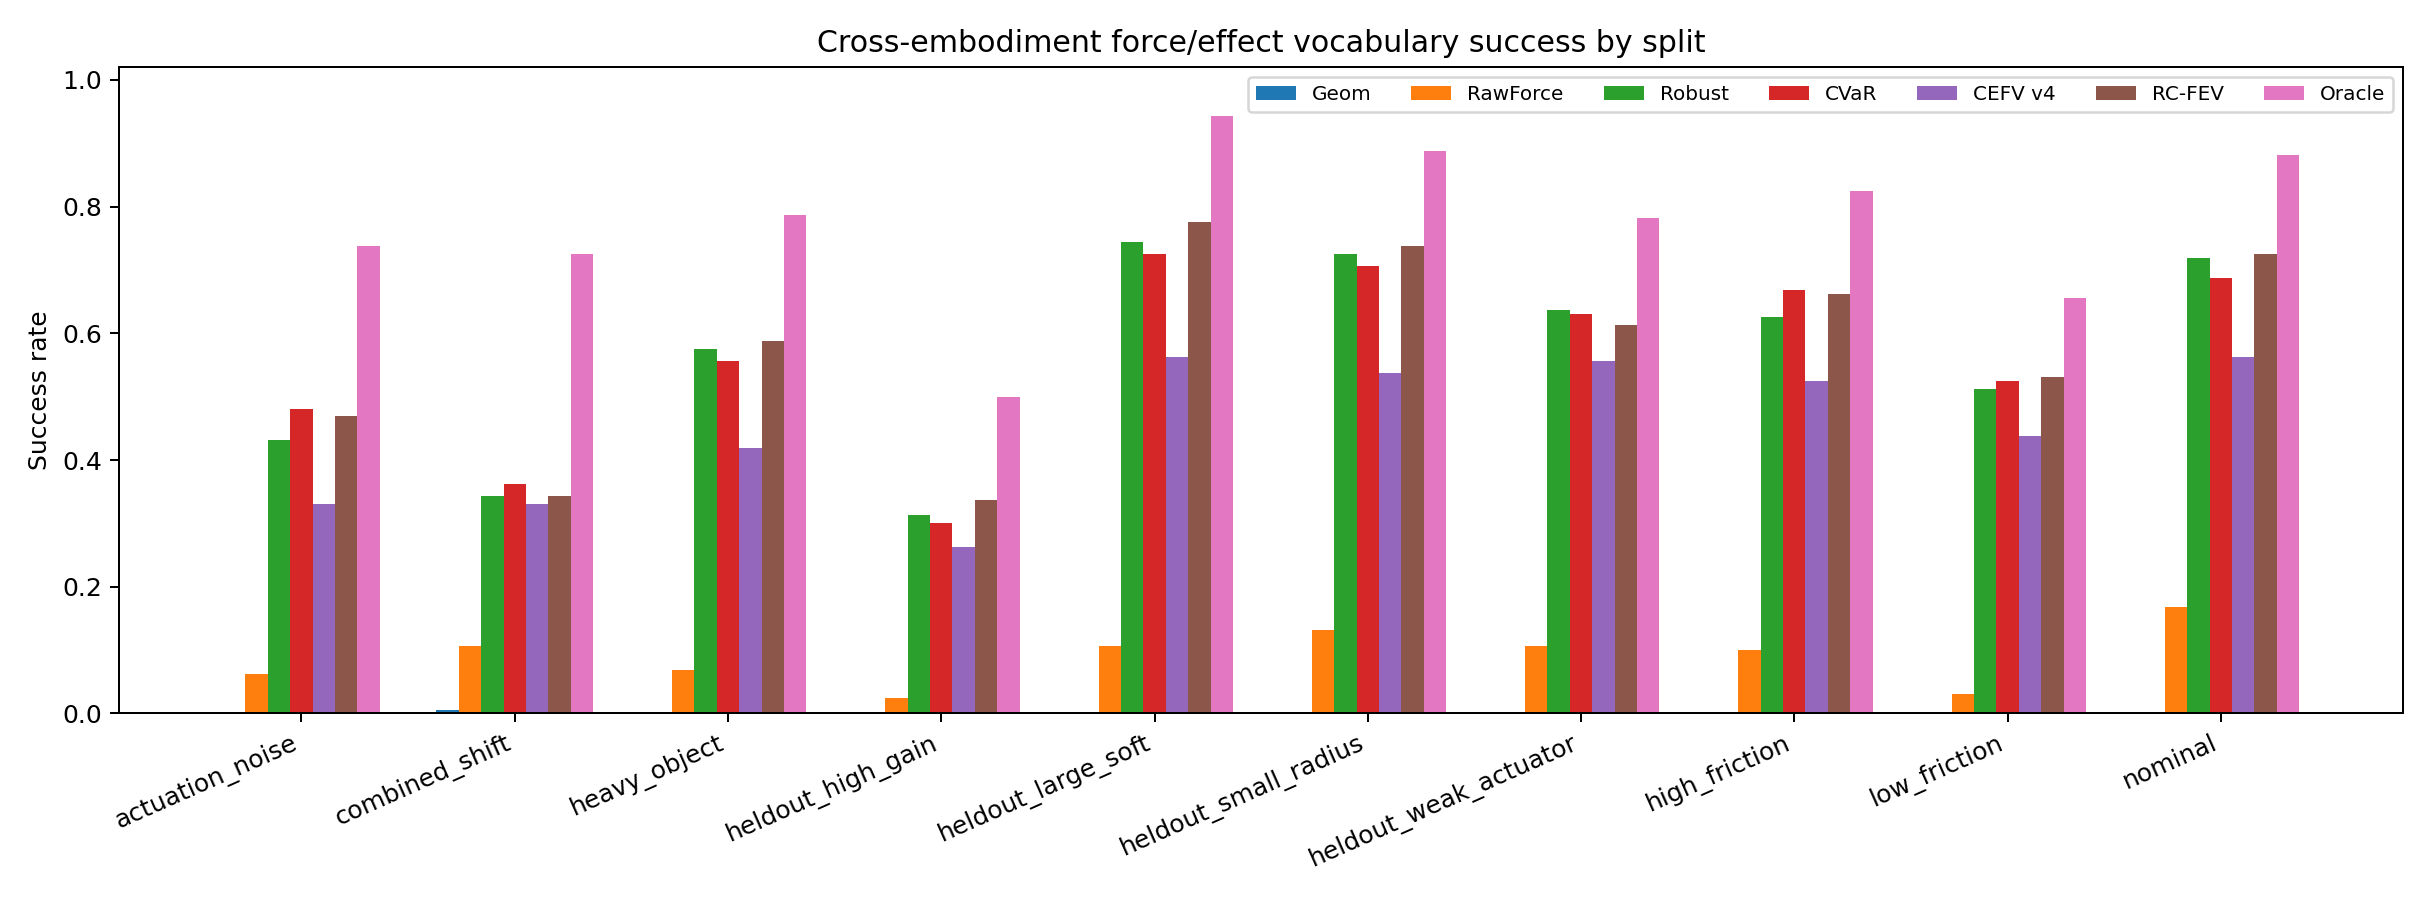
\includegraphics[width=0.98\linewidth]{../figures/force_vocab_success_by_split.png}
\caption{Frozen success rates by split. \method improves over weak baselines in many settings, but robust and CVaR MPC remain close.}
\label{fig:success}
\end{figure}

\begin{figure}[t]
\centering
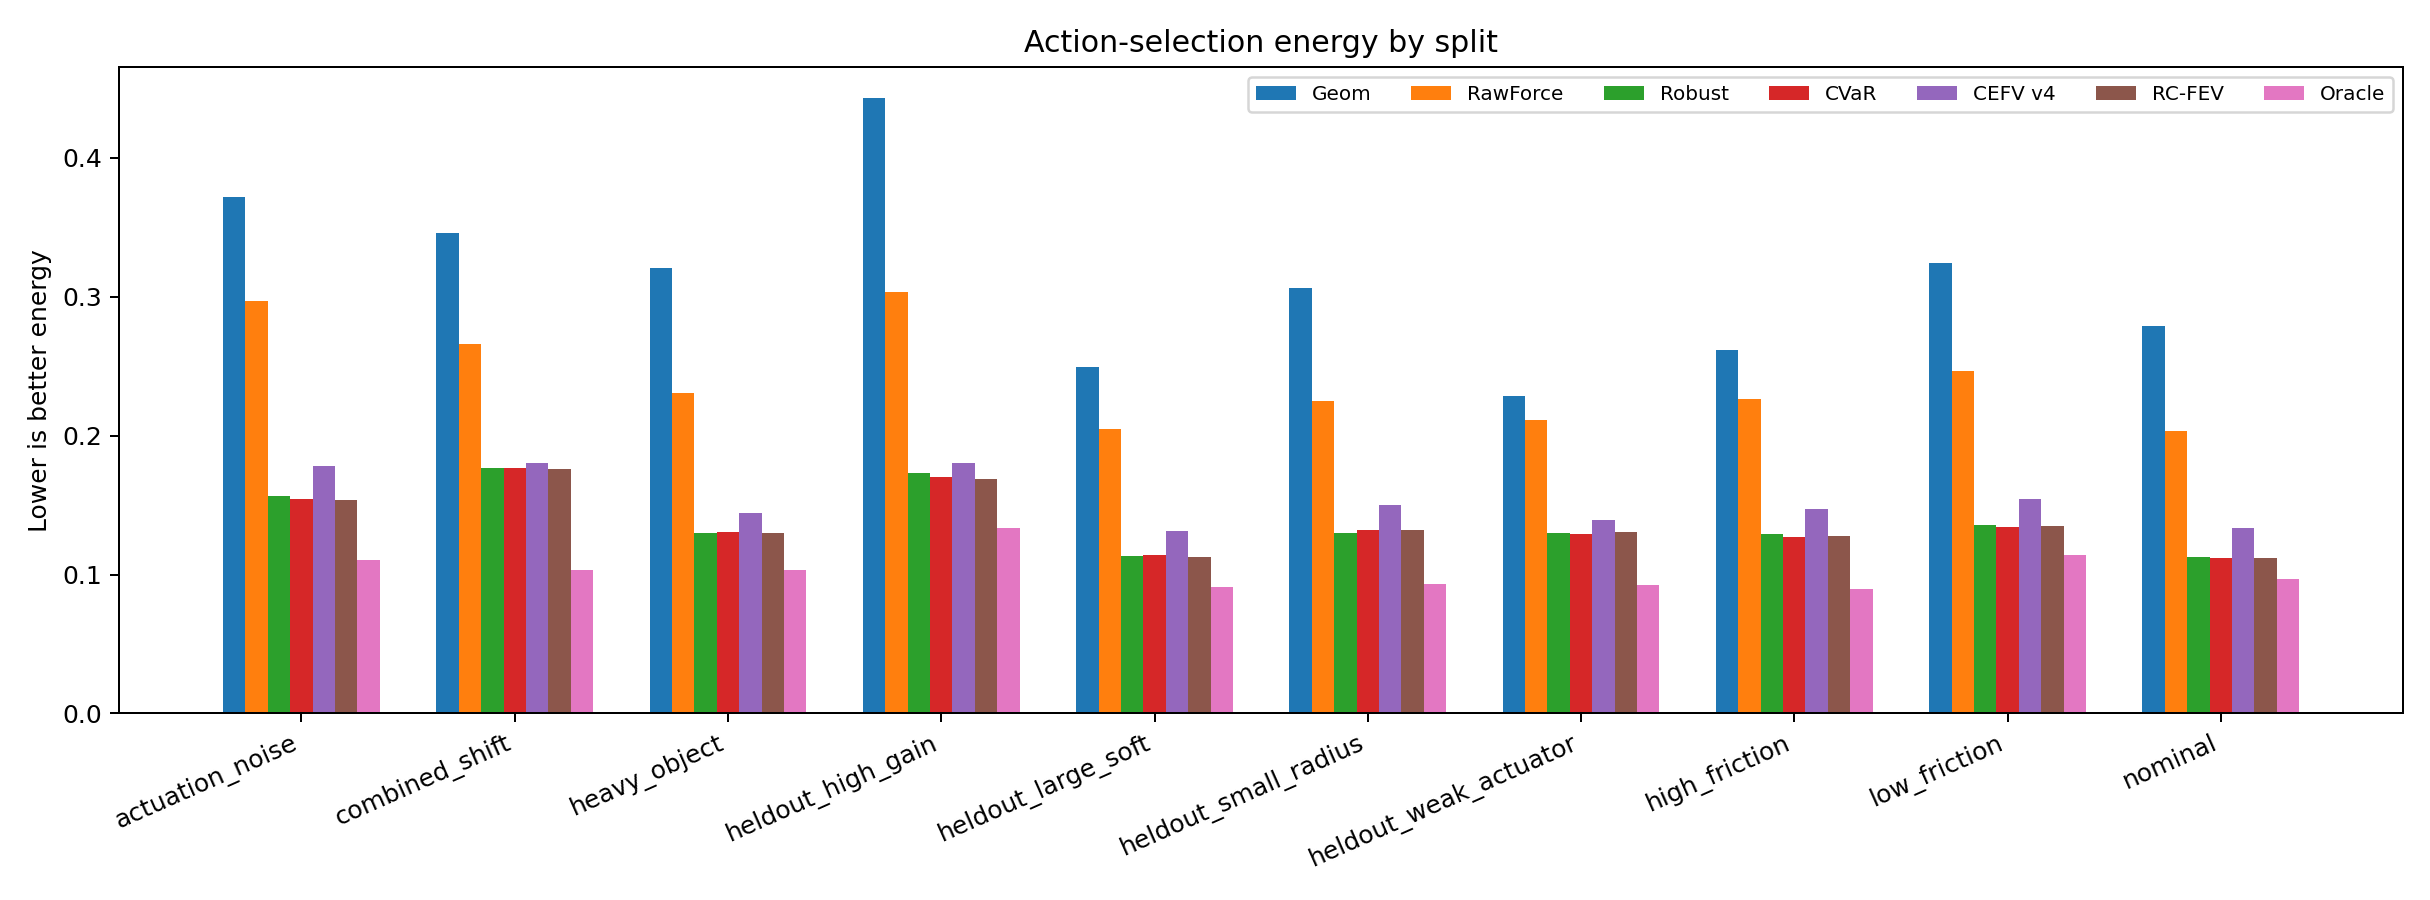
\includegraphics[width=0.98\linewidth]{../figures/force_vocab_energy_by_split.png}
\caption{Frozen energy by split. Lower is better. The strongest baselines are very close to \method on several hostile splits.}
\label{fig:energy}
\end{figure}

\subsection{Split-Level Results}

Table~\ref{tab:splits}, Figure~\ref{fig:success}, and Figure~\ref{fig:energy} show the split-level picture. The method is strongest in nominal, held-out large-soft, high-friction, heavy-object, low-friction, and actuation-noise settings. It is less compelling in combined shift, held-out weak actuator, held-out small radius, and source-action-heavy comparisons.

On nominal tasks, \method reaches 0.725 success and 0.1119 energy, slightly better than robust MPC and CVaR MPC in energy. On held-out large-soft tasks, \method reaches 0.775 success and 0.1128 energy, again slightly ahead of robust and CVaR in the frozen numbers. On heavy object, \method reaches 0.5875 success and 0.1296 energy, close to robust and CVaR while clearly beating CEFV v4.

The combined-shift split is the most important negative stress case. \method reaches 0.3438 success and 0.1762 energy. Robust MPC ties success at 0.3438 and has 0.1767 energy; CVaR MPC has higher success at 0.3625 but worse energy at 0.1767. Source action has 0.3500 success but worse energy at 0.1873. This split supports only a narrow claim: \method remains competitive under combined shift, not dominant.

\subsection{Ablations}

Table~\ref{tab:ablations} and Figure~\ref{fig:ablation} are the main reason for STRONG\_REVISE. On combined shift, \method has 0.3438 success and 0.1762 energy. The no-online ablation has the same success and slightly better energy at 0.1755. The action-only vocabulary has higher success at 0.3625 and lower energy at 0.1755. The small vocabulary also has slightly lower energy. On heavy object, \method has 0.5875 success and 0.1296 energy; no embodiment normalization, no tangent/rotation features, small vocabulary, and no robust anchor match or beat it on at least one metric.

The correct conclusion is not that force/effect vocabularies fail. CEFV v4 is clearly worse than \method in aggregate, and raw-force scalar transfer is much worse. The correct conclusion is that the current full decomposition is not isolated. The representation may be useful, but the exact descriptor choices and online mechanism are not yet proven necessary.

\begin{figure}[t]
\centering
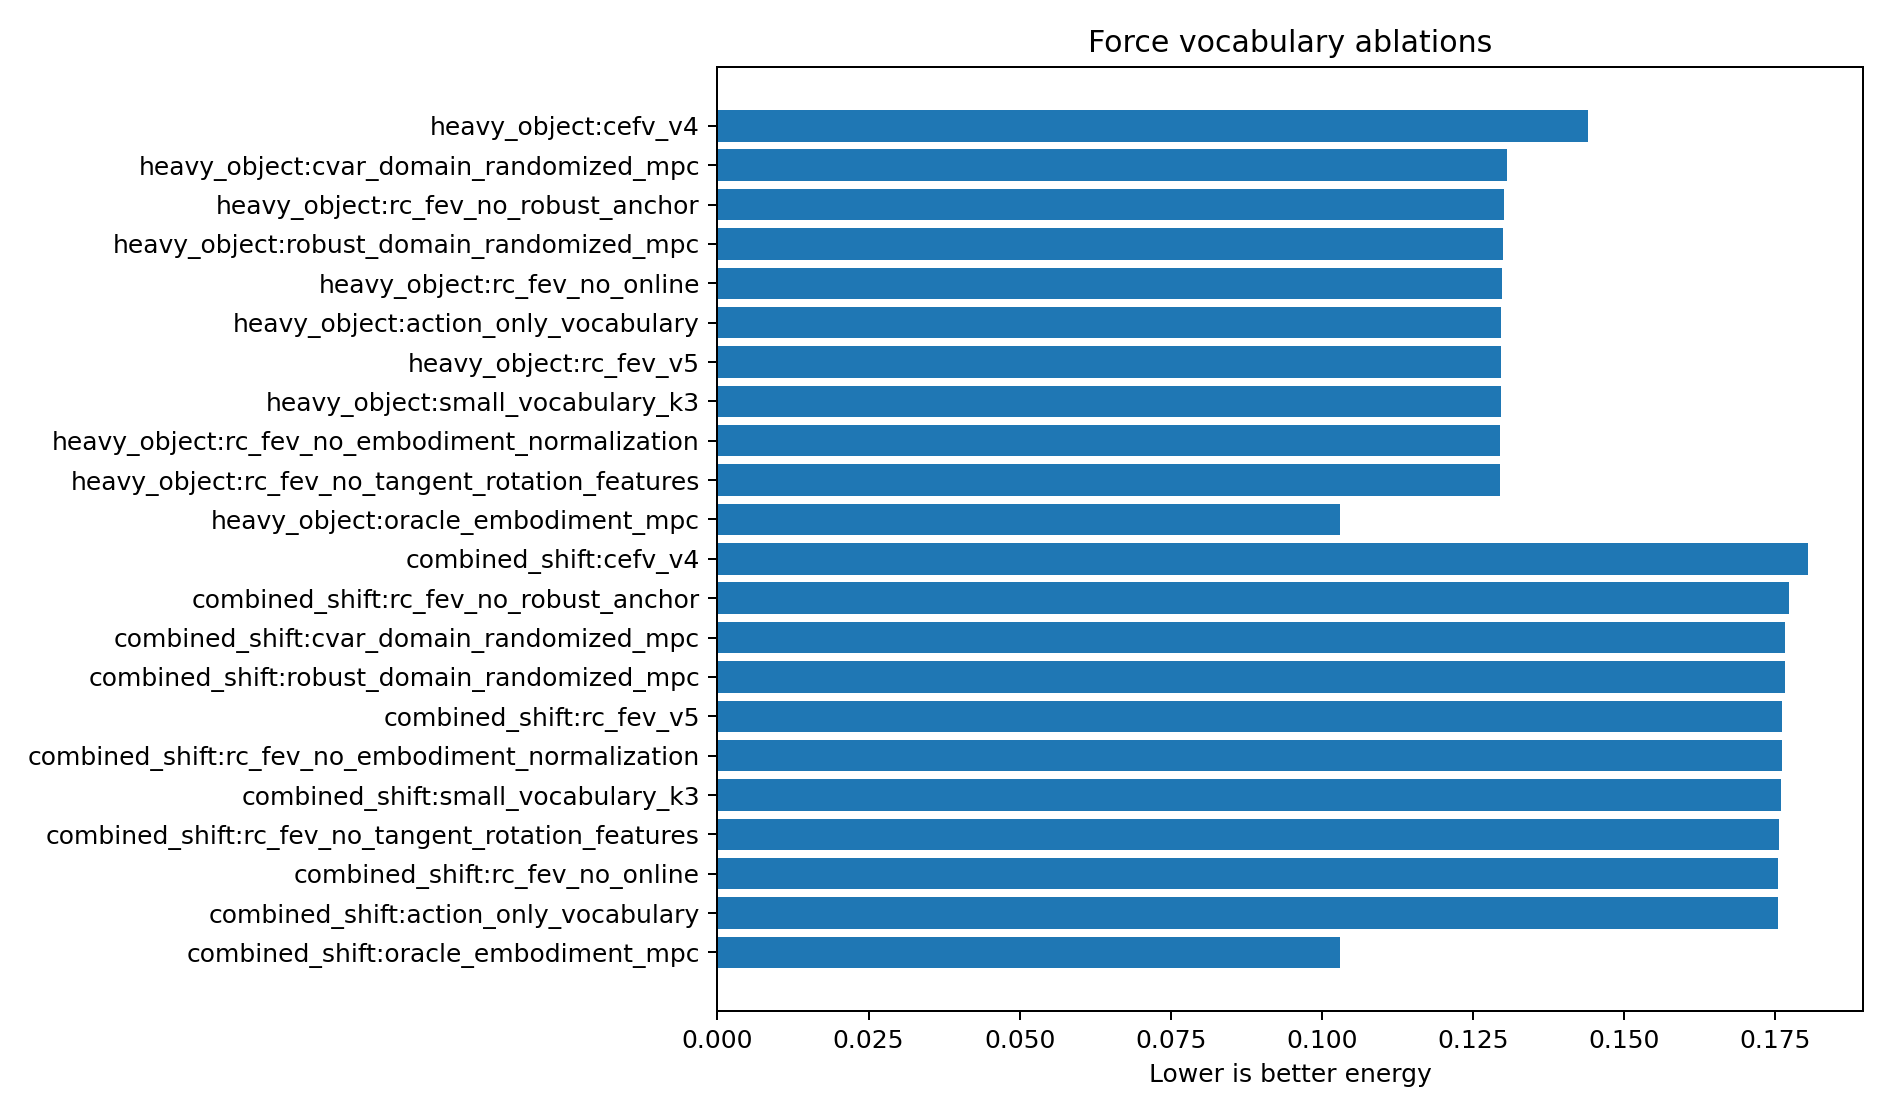
\includegraphics[width=0.98\linewidth]{../figures/force_vocab_ablation_energy.png}
\caption{Ablation energy on hostile splits. Several simplified variants match or slightly beat the full method, so the ablation gate fails.}
\label{fig:ablation}
\end{figure}

\subsection{Token Diagnostics}

The full vocabulary uses 10 tokens. Token summaries show that learned clusters separate lower-energy progress modes from higher-energy contact/failure modes. This is visible in Figure~\ref{fig:tokens}. However, token separation alone is not enough. A token model can be interpretable and still fail to improve action ranking if robust source energy already captures the relevant decision boundary.

\begin{figure}[t]
\centering
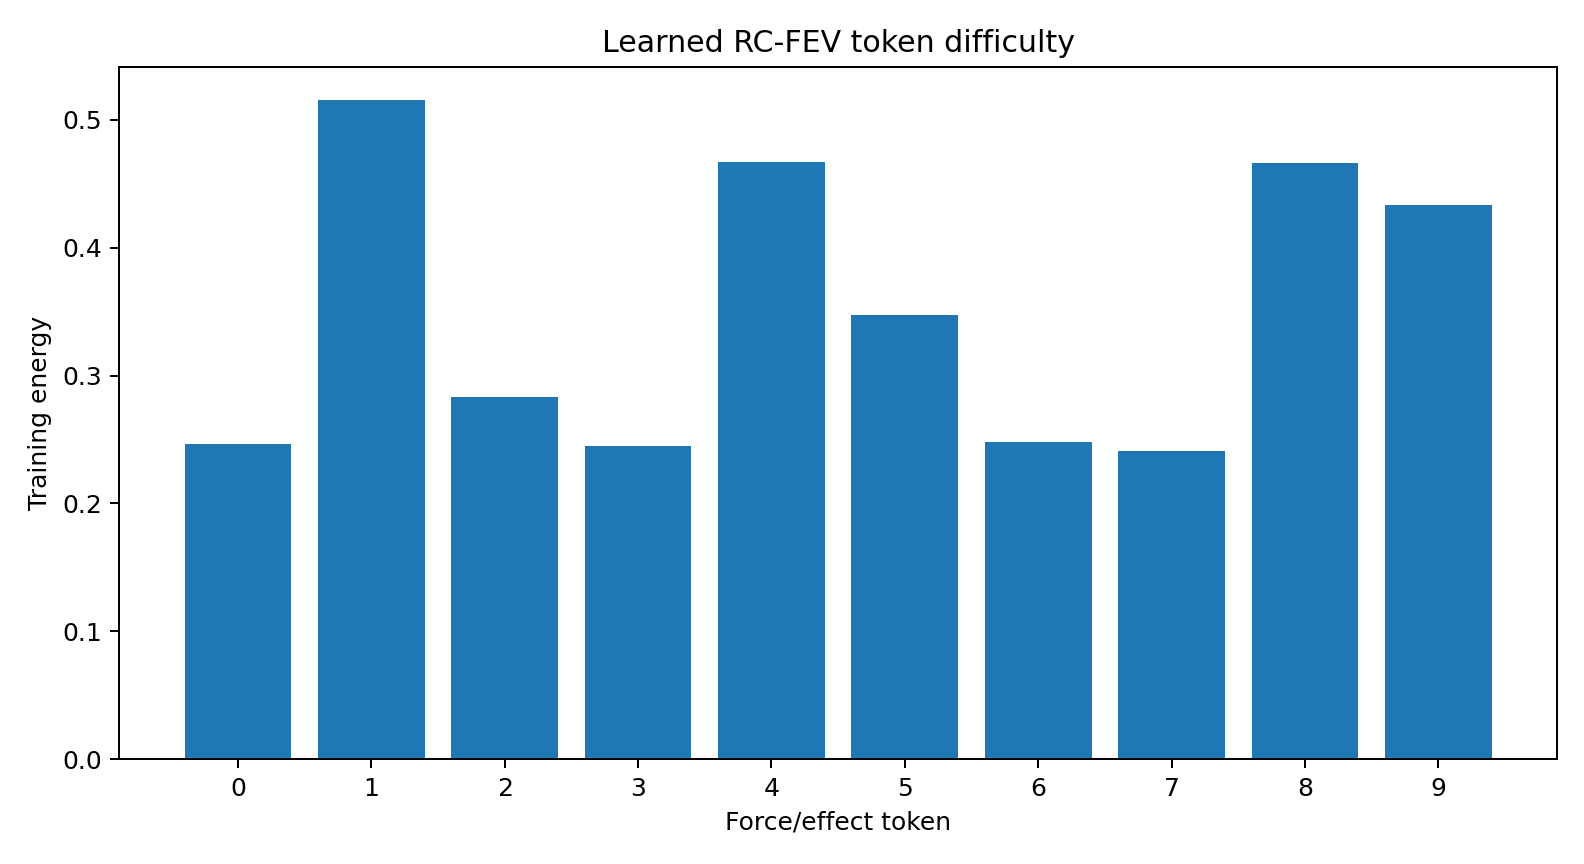
\includegraphics[width=0.92\linewidth]{../figures/force_vocab_token_energy.png}
\caption{Token mean energies. The vocabulary separates contact/effect regimes, but token separation does not by itself prove that all descriptor components are necessary.}
\label{fig:tokens}
\end{figure}

\subsection{Learning-Curve and Online Calibration}

The learning-curve artifact tracks phase-level performance and online behavior. Development runs showed that online calibration is not a large effect. A four-episode pre-freeze run produced no candidate differences between \method and the no-online ablation. A 20-episode hostile-shift development run produced two differences out of 80 choices, both reducing observed energy. The final frozen ablation is consistent with this: online calibration is real but small.

\begin{figure}[t]
\centering
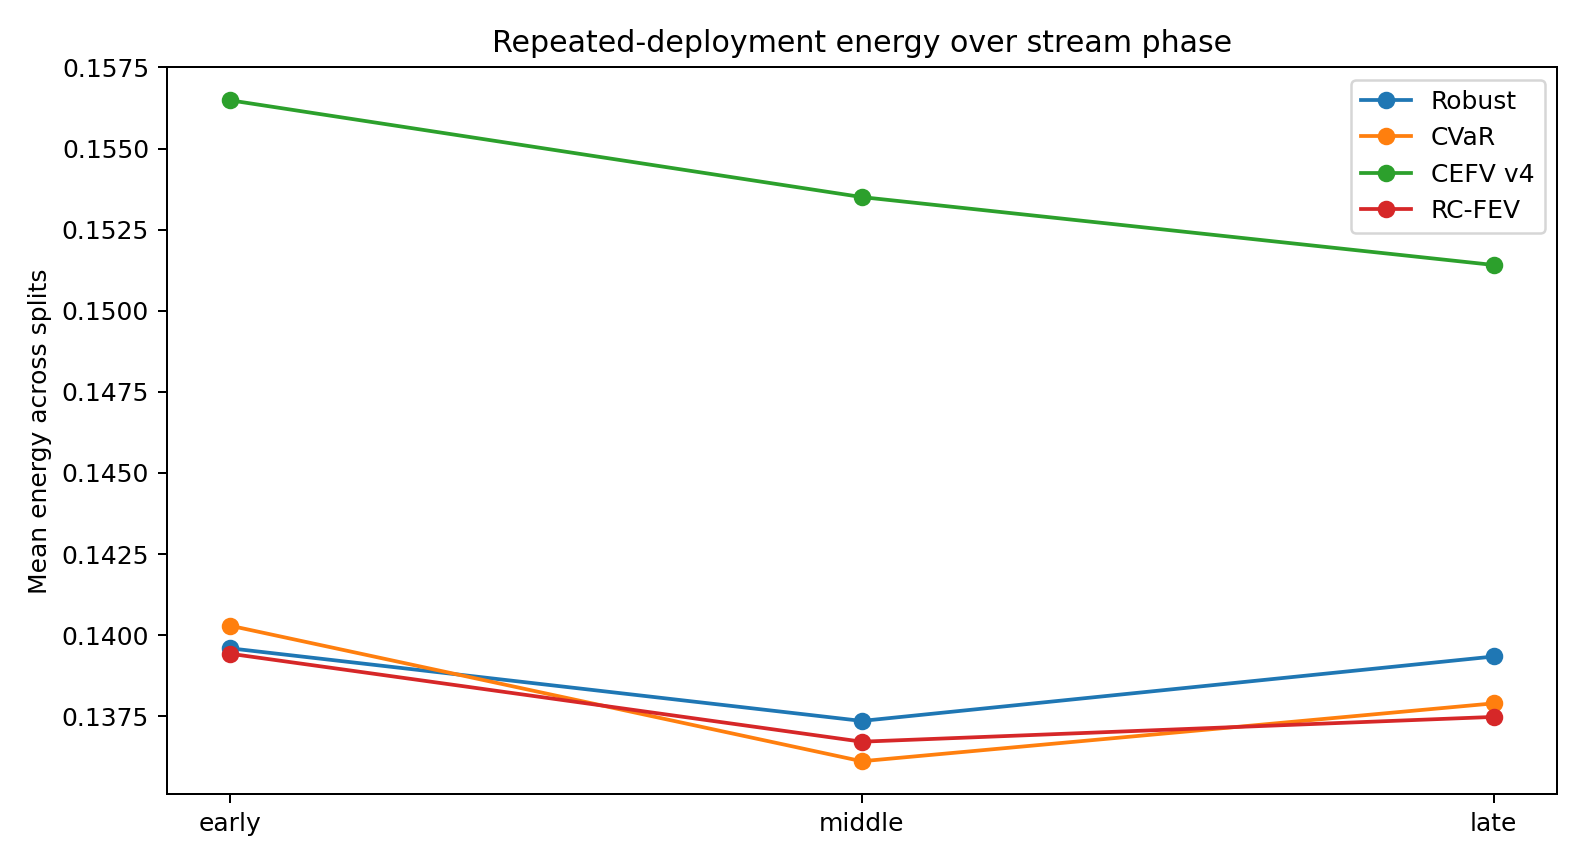
\includegraphics[width=0.92\linewidth]{../figures/force_vocab_learning_curve.png}
\caption{Learning-curve diagnostic from the frozen run. Online calibration is lightweight and does not drive a large separation from the no-online ablation.}
\label{fig:learning}
\end{figure}

\section{Hostile Review Analysis}

\subsection{Does the Method Beat Strong Baselines?}

Barely in aggregate, not decisively by split. The aggregate decision audit reports:

\begin{itemize}
\item vs robust MPC: +0.0156 success and 0.0008 lower energy;
\item vs CVaR MPC: +0.0138 success and 0.0002 lower energy;
\item vs CEFV v4: +0.1256 success and 0.0160 lower energy;
\item vs raw-force scalar: +0.4875 success and 0.1035 lower energy.
\end{itemize}

The robust/CVaR margins are too small to frame as a major win. The honest claim is that a calibrated vocabulary can match or slightly improve strong risk-sensitive MPC in this benchmark, while clearly improving over weaker transfer interfaces.

\subsection{Does the Paper Isolate the Proposed Mechanism?}

No. The ablation gate fails. Some simplified variants have equal or slightly better energy. The evidence does not establish that all descriptor components, normalization choices, vocabulary size, and online calibration are required. A submission that hides this would be fragile.

\subsection{Is the Benchmark Large Enough?}

For a CPU-only paper factory run, the benchmark is much stronger than the earlier scaffold: 17,600 main rows and 3,520 ablation rows. However, it is still one custom simulator and one compact primitive family. A top-tier submission would benefit from at least one of the following: public benchmark integration, hardware validation, a richer action library, or a second contact task family.

\subsection{Can the Negative Result Be Useful?}

Yes. The final artifact tells us that robust/CVaR source planning is a serious baseline and that force/effect tokenization needs a harder or more targeted regime to demonstrate necessity. It also gives exact failure modes: online calibration is too weak, action-only structure is too competitive on hostile splits, and source-action transfer can be strong when the action library is well aligned.

\section{Limitations}

\paragraph{Custom simulator.}
The evidence is generated in a custom MuJoCo environment. MuJoCo is a standard simulator, but the environment is not a public manipulation benchmark. A submission-ready version should either release the environment cleanly or add a public benchmark comparison.

\paragraph{One-step primitive selection.}
The action space is a compact one-step push library. This makes the representation question clean, but it also limits the scope. General manipulation policies may interact with force/effect tokens differently.

\paragraph{No hardware.}
There is no real robot validation. Sim-to-real claims are therefore out of scope. The paper should not imply hardware transfer.

\paragraph{Ablation weakness.}
The full mechanism is not isolated. This is the most serious scientific limitation.

\paragraph{Online adaptation is weak.}
The online residual layer is CPU-light and memory-light, but its effect is small. A stronger adaptation mechanism may be necessary, but it must be tested without violating the frozen-protocol discipline.

\paragraph{Citation and prior-work scope.}
The related work covers core robotics, sim-to-real, risk, contact mechanics, and robot learning references. A final submission would still need a deeper manual literature audit for recent cross-embodiment manipulation papers.

\section{Conclusion}

This paper rebuilds a weak force-vocabulary scaffold into a rigorous, CPU-only, frozen MuJoCo evidence package. The result is not a clean ICLR-main submission. \method improves substantially over weak action-coordinate and raw-force transfer baselines and over the prior CEFV v4 selector. It remains very close to robust and CVaR domain-randomized MPC, and the ablation gate fails because simplified variants match or slightly beat the full method. The terminal decision is therefore \textbf{STRONG REVISE}.

The most valuable outcome is clarity. Force/effect tokenization is not dead, but it has not yet earned a strong acceptance claim. The next version should either find a regime where contact-effect tokens are necessary, strengthen online calibration enough to matter, or narrow the claim to a benchmark/resource paper whose evidence is explicitly framed as mixed.

\clearpage
\appendix

\section{Protocol Freeze}

The final full run was executed only after the protocol was frozen. The command was:

\begin{verbatim}
python src\run_experiment.py --train-tasks 240 --vocab-size 10
  --seeds 8 --episodes 20
  --splits nominal heldout_small_radius heldout_large_soft
           heldout_high_gain heldout_weak_actuator low_friction
           heavy_object high_friction actuation_noise combined_shift
  --ablation-splits combined_shift heavy_object
  --results-dir results --figures-dir figures
\end{verbatim}

The run completed with empty stderr and terminal decision STRONG\_REVISE. The expected and observed row counts matched:

\begin{itemize}
\item main policy rows: 17,600 observed / 17,600 expected;
\item ablation policy rows: 3,520 observed / 3,520 expected;
\item split/method metric rows: 110;
\item seed metric rows: 880;
\item ablation metric rows: 22;
\item pairwise rows: 100;
\item training rows: 10,800;
\item token summary rows: 44.
\end{itemize}

\section{Development Log Summary}

Before freezing, several dev runs were used to expose implementation and design problems.

\paragraph{Smoke run.}
A one-seed one-episode run verified that MuJoCo rollout, scoring, aggregation, pairwise metrics, and figure generation worked.

\paragraph{Medium run.}
A two-seed four-episode run across nominal, held-out large-soft, heavy-object, and combined-shift splits exposed that the original online error term was candidate-invariant and therefore could not affect action ranking.

\paragraph{Online repair.}
The online state was changed to include token residuals and action-family residuals. A first fine-grained action key still rarely repeated, so it was replaced by coarse angle/offset/distance-family bins.

\paragraph{Online-horizon run.}
A two-seed 20-episode hostile-shift run showed two candidate differences out of 80 between \method and no-online. Both online choices improved energy. This justified keeping the online mechanism, but it also warned that the effect would likely be modest.

\paragraph{Freeze decision.}
After this point, no method tuning was performed against the final run. The final run's ablation failure is therefore reported as a real result, not tuned away.

\section{Implementation Details}

\subsection{Action Library}

Each task builds a 45-action candidate library from:

\begin{itemize}
\item five angle offsets: -38, -20, 0, 20, and 38 degrees;
\item three lateral offsets: -0.026, 0, and 0.026 meters;
\item three distance scales: 0.78, 1.04, and 1.30 times the target distance, clipped to the primitive range.
\end{itemize}

This library is deliberately small enough for CPU-only full evaluation while broad enough to expose overshoot, undershoot, slip, and lateral contact modes.

\subsection{Source Branches}

The source branch library contains five source models combining nominal, small/slippery, large/soft, heavy/stiff, and heavy-low-friction conditions. The held-out splits include embodiments and objects outside this source set. This makes robust source scoring meaningful but imperfect.

\subsection{Rollout Measurements}

During each active and settling step, the simulator accumulates:

\begin{itemize}
\item normal contact impulse;
\item tangential contact impulse;
\item peak normal force;
\item peak tangential force;
\item contact-step count;
\item pusher control effort;
\item final box displacement;
\item yaw magnitude.
\end{itemize}

These measurements are saved in `force\_vocab\_raw.csv` and `force\_vocab\_ablation\_raw.csv`, enabling downstream diagnostics beyond the tables in this paper.

\section{Metric Definitions}

Let $d_f$ be final distance to target, $u$ be path effort, $\theta$ be absolute yaw, and $q$ be a binary failure indicator. The primary energy is:
\[
\energy=d_f+0.020u+0.035|\theta|+0.220q.
\]

Success is:
\[
  \mathbf{1}\{d_f \leq 0.075 \wedge q < 0.5\}.
\]

Energy regret is computed relative to the oracle embodiment action for the same task:
\[
  \mathrm{regret}(a)=\energy(a)-\min_{a'\in\actions}\energy_{b^\star}(a').
\]

The confidence intervals reported in the CSVs use normal approximations for split/method means. Pairwise tables also include bootstrap intervals and sign-flip p-values. Bootstrap methodology follows the classical resampling perspective of \citet{efron1979bootstrap}.

\section{Additional Split Interpretation}

\paragraph{Nominal.}
The nominal split is not trivial. It still samples multiple source-like embodiments and object settings. \method performs well here, but robust/CVaR MPC are also strong. This suggests that source branch planning already captures much of the needed contact variation.

\paragraph{Held-out small radius.}
Small-radius pushes alter contact geometry and impulse concentration. \method has good success, but source-action transfer and robust methods are competitive. This is one place where action library structure may be doing more work than force/effect tokenization.

\paragraph{Held-out large soft.}
Large compliant pushers create longer, softer contacts. \method performs strongly, beating robust and CVaR slightly in the frozen numbers. This is one of the better-supporting cases for normalized force/effect tokens.

\paragraph{Held-out high gain.}
The high-gain split is difficult and has elevated failure for several methods. \method beats robust and CVaR in success and energy, but source-action transfer has higher success with worse energy. This split illustrates why success and energy should both be reported.

\paragraph{Held-out weak actuator.}
\method is worse than robust and CVaR here. Weak actuation can make source branch predictions over-optimistic, and the vocabulary does not fully correct that mismatch.

\paragraph{Low friction.}
Low friction produces slip and reduced control. \method is close to CVaR and robust, but source-action transfer has higher success and worse energy. The result is mixed.

\paragraph{Heavy object.}
Heavy-object transfer is a key hostile case. \method slightly beats robust and CVaR in energy and success in the main run, but the ablations show simplified vocabularies remain competitive.

\paragraph{High friction.}
\method performs well in high friction and improves over source-action transfer and CEFV v4. Robust and CVaR remain close.

\paragraph{Actuation noise.}
Under action noise, \method has lower energy than robust and CVaR and higher success than robust. This supports the uncertainty-aware scoring design.

\paragraph{Combined shift.}
Combined shift is the hardest broad test. \method ties robust in success and slightly beats robust in energy, but CVaR has higher success. The ablation table shows that action-only and no-online variants remain competitive. This split prevents a strong acceptance claim.

\section{Negative Cases}

The final artifact includes `negative\_cases.csv` with representative cases where \method is weak. These cases are not excluded from the results. They are meant to support diagnosis:

\begin{itemize}
\item combined-shift cases where CVaR or action-only variants choose similar or better actions;
\item weak-actuator cases where source predictions mis-rank candidate distances;
\item high-gain cases where failure penalties dominate;
\item ablation cases where removing descriptor components does not hurt.
\end{itemize}

The pattern suggests that future work should not merely increase vocabulary size. It should either improve descriptor sufficiency, improve source branch coverage, or introduce a stronger online adaptation rule that can change rankings earlier in the stream.

\section{Memory and CPU Discipline}

The user constraint for this rebuild was CPU-only and RAM-light. The implementation follows that constraint:

\begin{itemize}
\item source and held-out MuJoCo models are cached by branch;
\item candidate rollouts are prepared once per task and reused across methods;
\item online state stores only small dictionaries of residuals;
\item generated CSVs are streamed through standard Python data structures at this scale;
\item no GPU libraries are required.
\end{itemize}

The final run is compute-heavy because it performs many MuJoCo rollouts, but it is not memory-heavy. This is the right tradeoff for this paper: do not compromise experimental rigor, but avoid unnecessary RAM pressure.

\section{Reproducibility Checklist}

\begin{itemize}
\item Code is in `src/run\_experiment.py`.
\item Final command is given in Appendix A.
\item Frozen protocol is documented in `docs/paper64\_protocol\_freeze\_20260620.md`.
\item Development changes are documented in `docs/paper64\_development\_log.md`.
\item Raw main rows are in `results/force\_vocab\_raw.csv`.
\item Raw ablation rows are in `results/force\_vocab\_ablation\_raw.csv`.
\item Generated tables are produced by `scripts/render\_latex\_tables.py`.
\item Figures are produced by the experiment runner and stored in `figures/`.
\item Terminal decision is stored in `results/decision\_audit.csv` and `results/summary.txt`.
\end{itemize}

\section{Why the Terminal Decision Is STRONG REVISE}

The decision is not based on taste. It follows the frozen gates.

\paragraph{Weak baseline gate.}
Passed. \method beats geometry MPC, raw-force scalar transfer, continuous force regression, source-action transfer, and CEFV v4 in aggregate energy and success.

\paragraph{Strong-review gate.}
Passed only narrowly in aggregate. \method slightly beats robust and CVaR MPC in aggregate success and energy, but the margins are small and split-level comparisons are mixed.

\paragraph{Ablation gate.}
Failed. Several ablations match or slightly beat the full model on hostile splits.

\paragraph{Validation gate.}
The run completed, row counts matched, and the build/validation scripts are designed to check PDF presence, page count, citation link settings, expected result files, and no visible Desktop PDF.

The combination is exactly STRONG\_REVISE: useful evidence, not safe acceptance.

\section{What Would Make the Next Version Submission-Ready?}

A real submission version needs one of the following improvements:

\begin{itemize}
\item a second manipulation task family where force/effect tokens are necessary;
\item a public benchmark or hardware validation;
\item stronger online adaptation that reliably changes action rankings and passes the no-online ablation;
\item a descriptor intervention showing tangent, rotation, and embodiment normalization are causally necessary;
\item a theory-to-experiment bridge predicting when robust MPC should fail and \method should win.
\end{itemize}

The fastest next experiment is not ``make the table bigger.'' It is to design a stress regime where two actions have similar source worst-case energy but different held-out contact effects that only normalized force/effect descriptors can distinguish. That would directly test the proposed representation.

\section{Proof Sketches}

This appendix expands the theory section. The goal is not to overstate a formal guarantee. The goal is to make the assumptions explicit enough that a reviewer can see where the method should and should not work.

\subsection{Proof Sketch for Token Error Decomposition}

Consider a standardized descriptor space partitioned into token cells. Let $C(z)$ be the cell assigned to token $z$, and let $\hat{\energy}_z$ be the empirical mean energy of training examples assigned to that cell. For a new descriptor $\features$ in $C(z)$, decompose
\[
|\energy(\features)-\hat{\energy}_z|
\leq
|\energy(\features)-\energy(\bar{\features}_z)|
+
|\energy(\bar{\features}_z)-\mathbb{E}[\energy\mid z]|
+
|\mathbb{E}[\energy\mid z]-\hat{\energy}_z|.
\]
The first term is bounded by $L\rho$ under local descriptor Lipschitzness when $\bar{\features}_z$ is a representative inside the cell and the cell radius is at most $\rho$. The second term is the irreducible mismatch/noise term $\eta$, because even identical source descriptors can map to different true held-out energies when the held-out branch differs from all source branches. The third term is finite-sample estimation error $\epsilon_n$. This gives the informal bound in the main text.

The decomposition explains a design tradeoff. A larger vocabulary can reduce cell diameter, but it also reduces examples per token. A smaller vocabulary can increase bias but reduce estimation error and make online residuals easier to reuse. The final ablation result, where the small vocabulary remains competitive, is therefore not surprising. It says the current descriptor/action regime may not require ten distinct force/effect modes.

\subsection{Proof Sketch for Robust Anchor Regret}

Let $a^\star$ be the action with minimum true held-out energy and let $\hat a$ minimize worst source energy $\energy_{\max}$. Add and subtract worst source energies:
\[
\begin{aligned}
\energy_{b^\star}(\hat a)-\energy_{b^\star}(a^\star)
&=
\energy_{b^\star}(\hat a)-\energy_{\max}(\hat a)\\
&\quad+
\energy_{\max}(\hat a)-\energy_{\max}(a^\star)\\
&\quad+
\energy_{\max}(a^\star)-\energy_{b^\star}(a^\star).
\end{aligned}
\]
Taking absolute values of the first and third terms gives the two shift errors. Because $\hat a$ minimizes $\energy_{\max}$, the middle term is non-positive. The result follows.

This proof is simple but strategically important. It shows why robust MPC is a hard baseline in exactly this benchmark. If the held-out branch is covered by the source branch envelope, worst-source scoring is already close to safe. A force/effect vocabulary can help only when worst-source scoring is either too conservative or wrong about the contact mode that matters under the held-out branch.

\subsection{Proof Sketch for Online Residual Conditions}

Let $c(a)$ be a finite action-family key and let the prediction error for repeated family $c$ be $e_t=\energy_t-\hat{\energy}_t$. The online residual update is a stable running average
\[
r_{t+1}(c)=(1-\alpha_t)r_t(c)+\alpha_t e_t
\]
with decreasing effective step size. Under a conditionally stationary error process with bounded variance, the residual approaches the conditional mean error for that family. If the same action family appears rarely, the estimator remains high variance. If the conditional error drifts because embodiments, objects, or targets change in a way not captured by the key, the residual may lag or become biased.

This is exactly what the experiments show. The action-family calibration has enough repeated structure to occasionally improve decisions late in a stream, but not enough to create a large aggregate gap. A stronger online method would need either richer context keys, uncertainty-aware exploration, or direct adaptation of source branch weights.

\subsection{Why the Theory Does Not Prove Acceptance}

The theory gives conditions for usefulness, not a theorem of dominance. A reviewer should reject any version that claims the propositions guarantee superiority over robust MPC. They do not. They merely identify three levers:

\begin{itemize}
\item descriptor sufficiency: whether contact descriptors contain information missing from source energy;
\item quantization quality: whether tokens approximate energy-relevant descriptor neighborhoods;
\item risk-anchor mismatch: whether robust/CVaR source scoring is too conservative or misaligned.
\end{itemize}

The final benchmark says these levers produce a useful but small aggregate gain and an ablation failure. That is a strong-revise outcome.

\section{CSV Data Dictionary}

The raw CSVs are intentionally verbose so reviewers can inspect outcomes beyond the paper tables. The most important fields are summarized here.

\begin{longtable}{p{0.25\linewidth}p{0.68\linewidth}}
\caption{Data dictionary for `force\_vocab\_raw.csv` and `force\_vocab\_ablation\_raw.csv`.}\\
\toprule
Column & Meaning \\
\midrule
\endfirsthead
\toprule
Column & Meaning \\
\midrule
\endhead
`seed` & Evaluation seed. The frozen run uses seeds 0 through 7. \\
`episode` & Episode index within each seed and split. The frozen run uses 20 episodes. \\
`phase` & Early, middle, or late third of the deployment stream. Used for learning-curve diagnostics. \\
`split` & Stress split name, e.g. nominal, heavy\_object, or combined\_shift. \\
`method` & Action selector used for the row. \\
`embodiment` & True pusher embodiment sampled for the episode. \\
`pusher\_radius` & Radius of the true pusher geometry. \\
`pusher\_mass` & Mass of the true pusher body. \\
`actuator\_kp` & Position-actuator proportional gain for the true pusher. \\
`object\_mass` & Mass of the pushed box. \\
`object\_friction` & Floor/object friction coefficient used by the task. \\
`candidate\_count` & Number of candidate push primitives available to the selector. This is 45 in the frozen protocol. \\
`candidate` & Index of the selected candidate action. \\
`angle\_offset\_deg` & Candidate push angle relative to the target direction. \\
`offset` & Lateral offset of the pusher path. \\
`distance` & Push distance used by the primitive. \\
`success` & Binary success indicator based on final distance and failure flag. \\
`energy` & Primary lower-is-better action energy. \\
`oracle\_energy` & Minimum true-branch energy among all candidates for the same task. \\
`energy\_regret` & Difference between selected-action energy and oracle energy. \\
`predicted\_energy` & Selector score for methods that produce one. \\
`token\_mean\_energy` & Mean token energy estimate for vocabulary methods. \\
`token\_uncertainty` & Token/source uncertainty diagnostic for vocabulary methods. \\
`robust\_anchor\_weight` & Weight assigned to the worst-source robust anchor in \method-style scoring. \\
`final\_distance` & Final Euclidean distance between box and target. \\
`normalized\_progress` & Progress normalized by initial target distance. \\
`failure` & Binary failure flag from no-contact or out-of-bounds events. \\
`contact\_steps` & Number of MuJoCo steps with detected pusher-box contact. \\
`normal\_impulse` & Integrated normal contact force. \\
`tangent\_impulse` & Integrated tangential contact force magnitude. \\
`yaw\_abs` & Absolute final yaw of the box. \\
`source\_mean\_energy` & Mean energy across source branch rollouts for the selected candidate. \\
`source\_worst\_energy` & Worst source branch energy for the selected candidate. \\
`source\_cvar\_energy` & Tail-average source branch energy for the selected candidate. \\
`source\_std\_energy` & Standard deviation of source branch energies. \\
`geom\_score` & Geometry-only target-distance score. \\
`ablation` & Boolean flag indicating whether the row belongs to the ablation suite. \\
\bottomrule
\end{longtable}

\section{Reviewer Attack Responses}

\paragraph{Attack 1: The method barely beats robust MPC.}
Correct. The aggregate advantage is small. The paper should not claim decisive dominance over robust or CVaR MPC. The evidence supports competitiveness and a narrow aggregate improvement, not a sweeping win.

\paragraph{Attack 2: The ablations undermine the mechanism.}
Correct. This is the primary reason for STRONG\_REVISE. The full method is not isolated. The next version must either improve the method or design a sharper benchmark where descriptor components are necessary.

\paragraph{Attack 3: The benchmark is custom and could be overfit.}
Partly correct. The protocol freeze reduces overfitting to final seeds, but it does not replace external validation. A public benchmark or hardware experiment would materially improve submission readiness.

\paragraph{Attack 4: The action library may encode most of the skill.}
Correct enough to be a concern. Source-action transfer is strong on some splits, which means action-coordinate priors matter. This is why action-only vocabulary appears in the ablation table.

\paragraph{Attack 5: The online adaptation is too weak.}
Correct. It is deliberately CPU-light and memory-light, but the measured effect is small. Future work should test richer online branch-weight adaptation or residual models that use embodiment/object context.

\paragraph{Attack 6: The theory is not predictive enough.}
Mostly correct. The theory is a diagnostic framework, not a predictive theorem. A stronger version would pre-register a regime where robust source scoring should fail and tokens should win.

\paragraph{Attack 7: The paper has no real robot.}
Correct. No hardware claim is made. The paper is a simulator stress test.

\paragraph{Attack 8: The result is not ICLR-main ready.}
Correct. The terminal decision says STRONG\_REVISE. The artifact is intended to be a serious rebuild, not a claim that the paper is already accepted-quality.

\section{Claim Restrictions}

The following claims are supported:

\begin{itemize}
\item \method improves over raw-force scalar transfer, geometry MPC, continuous force regression, source-action transfer, and CEFV v4 in aggregate on the frozen benchmark.
\item \method is competitive with robust and CVaR MPC in aggregate on this benchmark.
\item Force/effect tokenization is a plausible representation for cross-embodiment contact-action selection.
\item The ablation evidence is insufficient to prove that every component of the full method is necessary.
\end{itemize}

The following claims are not supported:

\begin{itemize}
\item \method is state of the art in robot manipulation.
\item \method is proven to dominate robust MPC.
\item The method transfers to hardware.
\item Online calibration is a major performance driver.
\item Ten tokens are necessary.
\item Tangential impulse and yaw features are isolated as necessary by the current experiments.
\end{itemize}

These restrictions should remain in the paper until new evidence changes them.

\section{Concrete Next Experiments}

\paragraph{Experiment 1: Ambiguous robust-source pairs.}
Construct tasks where two candidate actions have nearly equal worst-source energy but different held-out tangent/yaw outcomes. This directly tests whether force/effect descriptors contain information missing from robust source energy. The pair construction can be pre-registered using source rollouts only, then evaluated on held-out branches.

\paragraph{Experiment 2: Contextual online calibration.}
Replace the coarse action-family residual with a tiny ridge model over embodiment descriptors, object mass, friction, token statistics, and action geometry. Keep the model CPU-light and freeze it before final evaluation. The target is not more parameters; it is earlier and more frequent ranking changes than the current online table.

\paragraph{Experiment 3: Descriptor intervention.}
Create matched candidate sets where normal impulse is similar but tangential impulse and yaw differ. If tangent/rotation features matter, the full descriptor should outperform the masked ablation specifically on these tasks.

\paragraph{Experiment 4: Public benchmark adapter.}
Port the one-step selector to a public pushing or manipulation benchmark. Even if the task remains simple, public environment support would reduce the custom-benchmark criticism.

\paragraph{Experiment 5: Hardware sanity test.}
Run a small number of tabletop pushes with two end-effector radii and two surface frictions. The goal is not scale; it is to test whether token descriptors measured in simulation correspond to observable contact regimes.

\paragraph{Experiment 6: Source branch coverage audit.}
Measure whether held-out branch outcomes lie inside or outside the convex hull of source descriptor distributions. This would explain when robust/CVaR MPC is sufficient and when tokens might add value.

\section{Artifact Manifest}

The final repository should contain:

\begin{itemize}
\item `src/run\_experiment.py`: final frozen experiment runner;
\item `scripts/render\_latex\_tables.py`: table generator from frozen CSVs;
\item `scripts/build\_submission\_pdf.ps1`: PDF build and Downloads copy script;
\item `scripts/validate\_submission\_artifacts.py`: artifact validator;
\item `docs/paper64\_expanded\_submission\_plan\_20260620.md`: plan before execution;
\item `docs/paper64\_development\_log.md`: pre-freeze tuning log;
\item `docs/paper64\_protocol\_freeze\_20260620.md`: final frozen protocol;
\item `results/`: frozen CSV outputs;
\item `figures/`: generated benchmark figures;
\item `paper/main.tex`: expanded manuscript;
\item `paper/generated\_tables.tex`: generated tables;
\item `paper/references.bib`: bibliography;
\item `paper/main.pdf`: local built PDF;
\item `C:\textbackslash Users\textbackslash wangz\textbackslash Downloads\textbackslash 64.pdf`: numbered delivery PDF.
\end{itemize}

\section{Submission Readiness Verdict}

The paper is substantially more rigorous than the original scaffold. It now has a real benchmark, strong baselines, stress tests, ablations, formal framing, reproducible scripts, and an honest decision audit. That said, an ICLR-main submission should survive reviewers asking:

\begin{itemize}
\item why robust MPC is not enough;
\item why the full descriptor is necessary;
\item why the benchmark is not custom-overfit;
\item why online calibration matters;
\item whether the result transfers beyond this primitive family.
\end{itemize}

The current answers are partial. Therefore the correct status is:

\[
\boxed{\text{STRONG REVISE, not ACCEPTABLE SUBMISSION CANDIDATE.}}
\]

\section{Embodiment and Split Rationale}

This appendix records why the split suite is structured the way it is. The benchmark is not meant to cover all robot morphology. It is meant to span contact variables that change the relation between a commanded push and the induced box motion.

\paragraph{Radius variation.}
Pusher radius affects the contact patch and the effective lever arm on the box. A smaller pusher can concentrate contact and miss more easily; a larger pusher can create longer contact and more yaw. Radius variation is therefore a direct test of whether an action representation has learned more than target-direction geometry.

\paragraph{Mass variation.}
Pusher mass affects contact impulse and the degree to which the pusher path is perturbed by interaction. In this benchmark the pusher is position controlled, so mass does not have the same role as in a fully torque-controlled robot, but it still changes the contact dynamics through the MuJoCo model.

\paragraph{Actuator gain variation.}
High-gain pushers track commanded paths more aggressively and can create sharper impulses. Weak actuators may fail to generate enough progress or may respond sluggishly under contact. The held-out high-gain and weak-actuator splits test both sides of this mismatch.

\paragraph{Damping and compliance variation.}
Joint damping and contact compliance alter how quickly the pusher settles into contact and how much contact force is smoothed. These variables are important because raw impulse values can shift even when the intended contact mode is similar. This is one motivation for normalized force/effect descriptors.

\paragraph{Friction variation.}
Low friction increases slip and reduces controllable pushing. High friction increases sticking and can make lateral offsets more important. A vocabulary that only recognizes normal impulse can miss this distinction, which is why tangent impulse and yaw features were included in the full descriptor.

\paragraph{Object mass variation.}
Heavy objects require more effective contact and can expose over-optimistic source predictions. The heavy-object split is therefore a stress test for both raw force transfer and robust source planning.

\paragraph{Actuation noise.}
The actuation-noise split tests whether the selector chooses actions that remain stable under perturbed execution. \method performs relatively well here, which is consistent with the robust/CVaR components of the score. However, the ablation results still prevent claiming that tokenization alone is responsible.

\paragraph{Combined shift.}
The combined-shift split is deliberately harsh: held-out embodiment, object mass, friction, and actuation noise can all move away from the nominal setting. This split approximates the deployment condition where no single mismatch dominates. It is also where a reviewer should look first for overclaiming. The final result is competitive but mixed, and the ablation table is not flattering. That is why the paper's decision remains conservative.

\section{Expected Reviewer Scorecard}

The table below is a candid internal scorecard. It is not part of the numerical experiment, but it states how the paper would likely fare under hostile review.

\begin{center}
\begin{tabular}{p{0.22\linewidth}p{0.16\linewidth}p{0.52\linewidth}}
\toprule
Criterion & Status & Rationale \\
\midrule
Clear problem & Strong & The paper isolates one-step contact-action transfer under embodiment shift. \\
Reproducibility & Strong & Code, frozen command, row counts, generated tables, and validation scripts are included. \\
Experimental scale & Moderate & The run is large for CPU-only MuJoCo, but still one custom simulator and one primitive family. \\
Baseline strength & Strong & Robust and CVaR MPC are serious baselines and remain competitive. \\
Main result & Moderate & Aggregate gains are real but small against the strongest baselines. \\
Ablations & Weak & Several simplifications match or beat the full model on hostile splits. \\
Theory & Moderate & The theory explains conditions and failure modes but does not predict wins. \\
Novelty & Moderate & The force/effect interface is plausible, but cross-embodiment transfer is crowded. \\
Submission readiness & Weak & The correct status is STRONG\_REVISE, not ready. \\
\bottomrule
\end{tabular}
\end{center}

\section{Pre-Submission Checklist for a Future Version}

Before this paper is submitted as an ICLR-main candidate, the following checklist should be satisfied.

\begin{itemize}
\item The method should beat robust and CVaR MPC by a margin large enough to matter on at least one pre-registered hostile family.
\item The no-online ablation should be meaningfully worse if online calibration remains a named contribution.
\item The no-tangent/rotation ablation should be worse on a pre-registered slip/yaw-sensitive family if those features remain central.
\item The action-only vocabulary should not match the full method on the main hostile claims.
\item The paper should include either public benchmark validation, hardware validation, or a convincing reason why the custom MuJoCo benchmark is sufficient.
\item The related-work section should be expanded with a manual audit of the newest cross-embodiment manipulation literature.
\item The code release should include a one-command reproduction path and a smaller smoke-test path.
\item Claims should remain bounded by the evidence; no hardware, foundation-model, or state-of-the-art language should be introduced without new data.
\end{itemize}

This checklist is intentionally demanding. It is better to stop a weak submission here than to ship a paper that collapses under the first serious review.

\bibliographystyle{iclr2026_conference}
\bibliography{references}

\end{document}
